\documentclass[letterpaper]{article} 
\usepackage[left = 0.5in, right = 0.5in, top = 0.9in, bottom = 0.9in]{geometry}
\usepackage{enumitem}
\usepackage{multicol}
\setlength{\multicolsep}{1cm}
\usepackage[spanish]{babel}
\usepackage[utf8]{inputenc}

\usepackage{amsmath,amssymb,amsthm}
\usepackage{tikz-cd}
\usepackage{mathrsfs}
\usepackage[bbgreekl]{mathbbol}
\usepackage{dsfont}
\usepackage{graphicx}
\usepackage{hyperref}
\graphicspath{{img/}}

\newcommand{\op}{\operatorname}
\newcommand{\Op}{^{\op{op}}}
\newcommand{\scc}{\mathscr C}
\newcommand{\scd}{\mathscr D}
\newcommand{\sce}{\mathscr E}
\newcommand{\sci}{\mathscr I}
\newcommand{\scj}{\mathscr J}
\newcommand{\scx}{\mathscr X}
\newcommand{\var}{\mathrm{Var}}
\newcommand{\Id}{\operatorname{Id}}
\newcommand{\N}{\mathbb N}
\newcommand{\Z}{\mathbb Z}
\newcommand{\Q}{\mathbb{Q}}
\newcommand{\I}{\mathbb{I}}
\newcommand{\R}{\mathbb{R}}
\newcommand{\C}{\mathbb{C}}
\newcommand{\F}{\mathcal{F}}
\newcommand{\G}{\mathcal{G}}
\newcommand{\B}{\mathcal{B}}
\newcommand{\abs}[1]{\left\lvert #1 \right\rvert}
\newcommand{\inv}{^{-1}}
\renewcommand{\to}{\rightarrow}
\newcommand{\ent}{\Longrightarrow}
\newcommand{\E}{\mathbb{E}}
\renewcommand{\P}{\mathbb{P}}
\newcommand{\1}{\mathds{1}}
\renewcommand{\qedsymbol}{$\blacksquare$}

\theoremstyle{definition}
\newtheorem{dfn}{Definición}
\theoremstyle{definition}
\newtheorem{teo}{Teorema}
\theoremstyle{definition}
\newtheorem{cor}{Corolario}
\theoremstyle{definition}
\newtheorem{prop}{Proposición}
\theoremstyle{definition}
\newtheorem{obs}{Observación}


\title{\textbf{Cómputo Científico\\ Tarea 5\\
Simulación Estocástica, introducción}}
\author{Iván Irving Rosas Domínguez}
\date{\today}

\DeclareSymbolFontAlphabet{\mathbbm}{bbold}
\DeclareSymbolFontAlphabet{\mathbb}{AMSb}
\DeclareMathSymbol\bbDelta  \mathord{bbold}{"01}

\begin{document}
\maketitle

%\begin{abstract}
%\end{abstract}

\begin{enumerate}
    \item[\textbf{1.}] Definir la cdf inversa generalizada $F_X^{-}$ y demostrar que en 
    el caso de variables aleatorias continuas esta coincide con la inversa usual. Demostrar
    además que en general para simular de $X$ podemos simular $u\sim U(0,1)$ y $F_X^{-}(u)$ se 
    distribuye como $X$. [1 punto]\\


    \textbf{Solución:} Comenzamos por la definición de inversa generalizada:
      \begin{dfn}(Inversa generalizada [por izquierda].) Sea $F$ una función de distribución. Definimos la 
        inversa generalizada de $F$, denotada por $F^{-}$, como 
        \[
        F^{-}:(0,1)\to \R, \qquad F^{-}(t):=\inf\{x\in R \ : \ F(x)\geq t\}.    
        \] 
        Notemos que esta función está bien definida en el dominio $(0,1)$ puesto que $F$ toma valores en $(0,1)$. 
        Además, dado que $F$ es continua a la derecha (es función de distribución) 
        el ínfimo anterior existe.
      \end{dfn}
      Tenemos ahora el siguiente teorema:
      \begin{teo}
        Sea $X$ una variable aleatoria con función de distribución $F$ estrictamente creciente y continua. Entonces 
        la inversa generalizada de $F$ coincide con su inversa verdadera.
      \end{teo}
      \begin{proof} 
        Notamos primero que $F$ tiene inversa real, ya que es una función monótona estrictamente creciente, y 
        además es una función continua, por lo que existe su inversa y de hecho su inversa es también 
        estrictamente creciente. Resta ver que coinciden en cualquier punto del intervalo $(0,1)$. Sea $t\in (0,1)$.
        Nótese que $F^{-1}(t)$ es una cota inferior del conjunto $A_t:=\{x\in R \ : \ F(x)\geq t\}$. En efecto, 
        sea $x\in A_t$, y nótese que
        \[
            x\in A_t \quad \ent \quad x\in \R \text{ y } F(x)\geq t \quad \Longleftrightarrow \quad x\geq F^{-1}(t),
        \]
        por lo que $F^{-1}(t)\leq x$, para cualquier $x\in A_t$. Resta ver que es la cota inferior mínima de $A_t$. 
        Para ello, supongamos que $x\in \R$ es una cota inferior de $A_t$. Si suponemos que $x>F^{-1}(t)$, entonces 
        existe $z\in \R$ tal que $x>z>F^{-1}(t)$, y dado que $F$ es estrictamente creciente, 
        \[
        x>z>F^{-1}(t) \quad \ent \quad F(x)>F(z)>F \left(F^{-1}(t)\right)=t,    
        \]
        es decir, $F(z)>t$ y por lo tanto $z\in A_t$. Pero teníamos que $x>z$, por lo que entonces $x$ no es una cota inferior
        del conjunto $A_t$, lo cual es una contradicción.\\

        Por lo tanto, $x\leq F^{-1}(t)$ y con ello, $F^{-1}(t)=\inf\{x\in \R \ : \ F(x)\geq t\}$, por lo que por definición de
        inversa generalizada,
        \[
        F^{-}_X(t)=F^{-1}(t).    
        \]
       \end{proof}
       Finalmente veamos que si conocemos la distribución $F$ de una variable aleatoria $X$, entonces
       podemos simular de ella a partir de una uniforme $u\sim U(0,1)$ y realizando $F_X^{-}(u)$. Lo anterior
       se puede traducir en el siguiente 
       \begin{teo}
        Sea $X$ una variable aleatoria con distribución $F_X$ y sea $u\sim U(0,1)$. Entonces 
        $F^{-}_X(u)$ tiene la misma distribución que $X$
       \end{teo}
       \begin{proof} 
         Claramente $F^{-}_X(u)$ es una nueva variable aleatoria y como tal, tiene una función 
         de distribución. Queremos ver que dicha función de distribución es $F_X$ misma, esto es,
         buscamos que para $t\in \R$,
         \[
         \P\left(F^{-}_X(u)\leq t\right)=F_X(t). 
         \] 
         Para lo anterior, probamos primero que para cualquier $t\in \R$, 
         \[
         \left\{F_X^{-}(u)\leq t\right\}=\left\{u\leq F_X(t)\right\}.
         \]
         Para ello, pensamos mejor en el complemento de los conjuntos, esto es, 
         \[
          \left\{F_X^{-}(u)> t\right\}=\left\{u> F_X(t)\right\}.
         \]
         $\subseteq)$ Nótese que si $\omega \in \left\{F^{-}_X(u)> t\right\}$, entonces 
         para cualquier $x\in \R$, $F_X(x)\geq u(\omega) \quad \ent \quad x>t$ por definición de ínfimo. Pero entonces si no fuera
         cierto que $\omega \in  \left\{u> F_X(t)\right\}$, se tendría que $F_X(t)\geq u(\omega)$ y por lo 
         tanto, $t>t$, lo cual es una contradicción.
         \newline

         $\supseteq)$ Supongamos ahora que $\omega \in \left\{u> F_X(t)\right\}$. Debemos
         probar que para cualquier $x\in \R$, $F_X(x)\geq u(\omega) \quad \ent \quad x>t$.
         Sea pues $x\in \R$ y supongamos que $F_X(x)\geq u(\omega)$. Entonces como $u(\omega)>F_X(t)$,
         se tiene que $F_X(x)>F_X(t)$, por lo que nuevamente, si no ocurriera que $x>t$, entonces
         $x\leq t$ y por ser $F$ monótona no decreciente, $F_X(x)\leq F_X(t)$, lo cual
         contradice lo anterior.
         
         Se puede concluir que $F^{-}_X(u(\omega))\geq t$, y para obtener la desigualdad estricta, 
         nótese que si $t=\inf\{x\in \R \ : \ F(x)\geq u(\omega)\}$, entonces podríamos seleccionar una
         sucesión $(h_n)_{n\geq0}\subseteq \{x\in \R \ : \ F(x)\geq u(\omega)\}$ tal que $h_n\to t$ por derecha, 
         y gracias a la continuidad de $F$ por derecha, se tendría que $u(\omega)\leq F(h_n)\to F(t)$, es decir, $u(\omega)\leq F(t)$, 
         lo cual nuevamente vuelve a contradecir el que $u(\omega)>F_X(t)$. 
         \newline

         Se tiene pues la igualdad de los conjuntos anteriores y por lo tanto de sus complementos. Esto significa que 
         \[
         \P\left(F_X^{-}(u)\leq t\right)=\P\left(u\leq F_X(t)\right),
         \]
         pero $u\sim U(0,1)$, por lo que 
         \[
         \P\left(u\leq F_X(t)\right) =F_X(t),
         \]
         es decir, 
         \[
          \P\left(F_X^{-}(u)\leq t\right)=F_X(t),
         \]
         y concluimos.
        \end{proof}

    \item[\textbf{2.}]Implementar el siguiente algoritmo para simular variables aleatorias 
    uniformes:
    \[
    x_i=107374182x_{i-1}+104420x_{i-5} \qquad (\text{mód} \ 2^{31}-1),
    \]
    regresa $x_i$ y recorrer el estado, esto es, $x_{j-1}=x_{j}$; $j=1,2,3,4,5;$ ¿parecen $U(0,1)$?[1 punto]\\

    \textbf{Solución:} Se implementó el algoritmo para simular uniformes en (0,1). El algoritmo en python se encuentra en el script \textit{Ejercicios 2-5}.
    En él, se encuentra definida una función denominada \textit{$gen\_unif$}. El script contiene comentarios
    donde se documenta la construcción de tal función.

    A grandes rasgos, dicha función toma dos argumentos, el primero $n$ corresponde 
    al número de muestras que se quieren crear con este algoritmo, y el segundo corresponde
    a un argumento que, si se le ingresa el valor $1$, entonces utilizará el vector
    \[
    X_0=\left(1111,3452,5642,5346,2454\right)
    \]
    como vector para iniciar el algoritmo. Dichos números fueron escogidos 
    al azar, pero son fijos. La finalidad de este es poder reproducir un ejemplo 
    con motivos de visualización.

    Por otro lado, si dicho argumento es distinto de 1, entonces el vector 
    con el que algoritmo inicia está dado por 
    \[
      X_0=\left(\text{semilla},3452,5642,5346,2454\right),
    \]
    donde \textit{semilla} es un valor que corresponde al tiempo cibernético, el 
    cual a cada segundo es distinto. Dicho valor se obtiene utilizando el comando \begin{verbatim}
      time.time()
    \end{verbatim} y posteriormente se transforma a entero.\\

    Como muestra del algoritmo, se realizan dos ejemplos. El primero de ellos sin 
    aleatoriedad y el segundo de ellos con aleatoriedad. Para el primero se 
    realiza una muestra de tamaño $n=100,000$. Se realiza un histograma de las muestras y 
    se contrasta en la misma gráfica con la densidad de una variable uniforme 
    en (0,1). Los resultados están presentes en las figuras 1 y 2.\\

    \begin{figure}[h!]
      \centering
      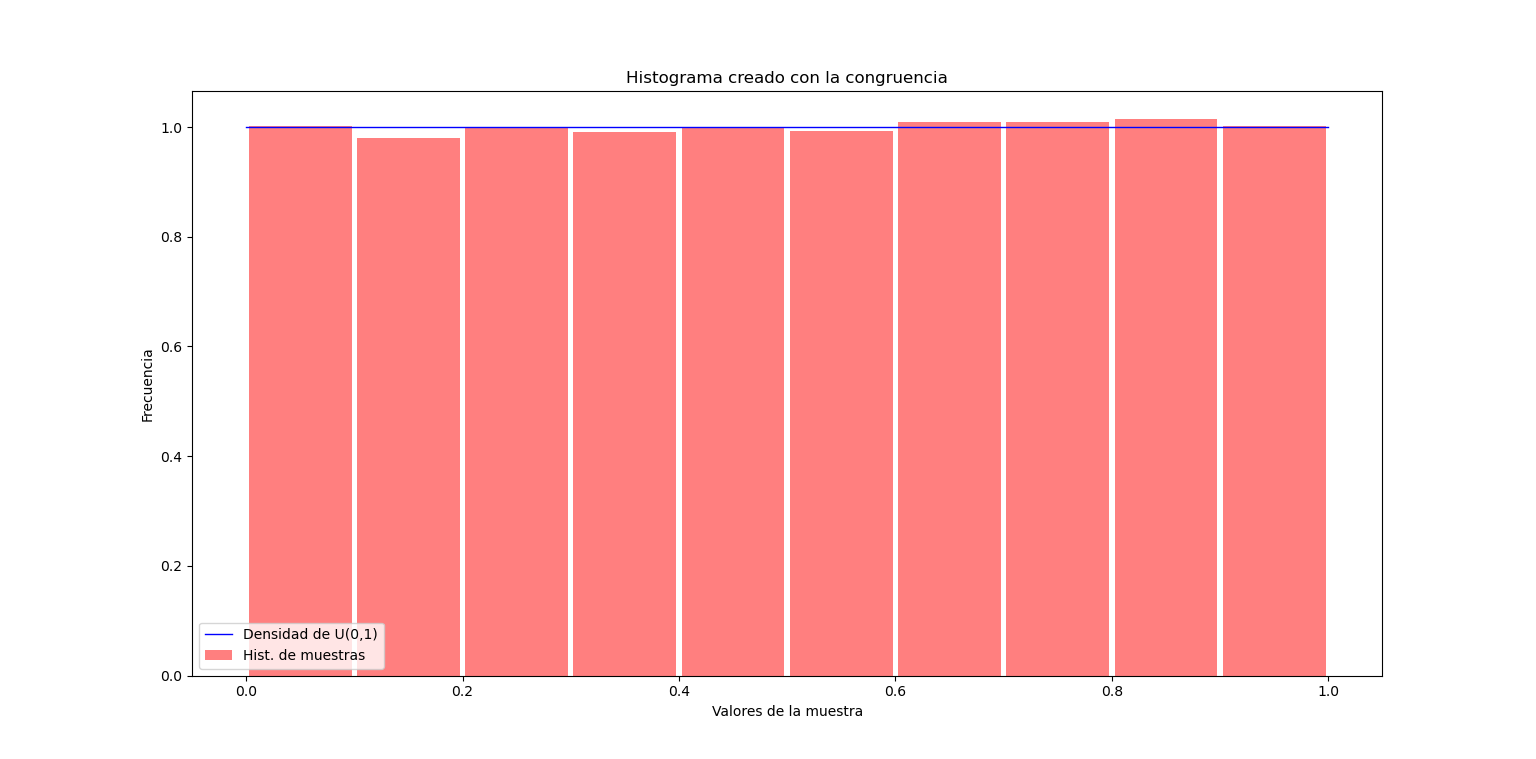
\includegraphics[width=0.9\linewidth]{1.png}
      \caption{Histograma de 100,000 muestras del algoritmo y su contraste con una densidad uniforme en (0,1). Vector inicial fijo.}
  \end{figure} 
  \begin{figure}[h!]
    \centering
    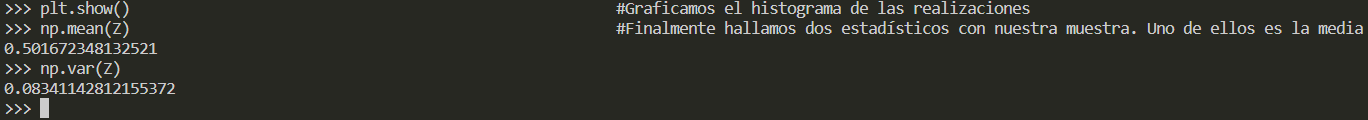
\includegraphics[width=0.9\linewidth]{2.png}
    \caption{Media y varianza del muestreo anterior.}
\end{figure} 

Obsérvese que el histograma aproxima notoriamente bien a la función de densidad que está 
graficada en color azul. Asimismo, podemos apreciar el resultado del cálculo 
de dos estadísticos de la muestra: uno de ellos es la media, el cual es un estadístico 
cuyo valor teórico es $\frac{1}{2}$, y que en nuestro caso, se tiene que $\widehat{\mu}\approx0.50167$,
el cual es bastante cercano al valor teórico.

Finalmente, el valor de la varianza muestral es de $\widehat{\sigma}^2\approx0.834114$, el 
cual también es bastante cercano al valor de la varianza teórica que está dado por $\frac{(1-0)^2}{12}=\frac{1}{12}=0.08333...$.
Los resultados anteriores muestran que esta muestra se comporta razonablemente como una muestra de 
variables aleatorias uniformes en (0,1).\\

Procedemos igualmente con el caso aleatorio. Se vuelve a realizar una muestra con $n=100,000$, y 
extraemos la muestra. Realizamos el histograma, contrastamos con la densidad uniforme, y calculamos 
la media y varianza muestrales. Los resultados están en las figuras 3 y 4.\\

\begin{figure}[h!]
  \centering
  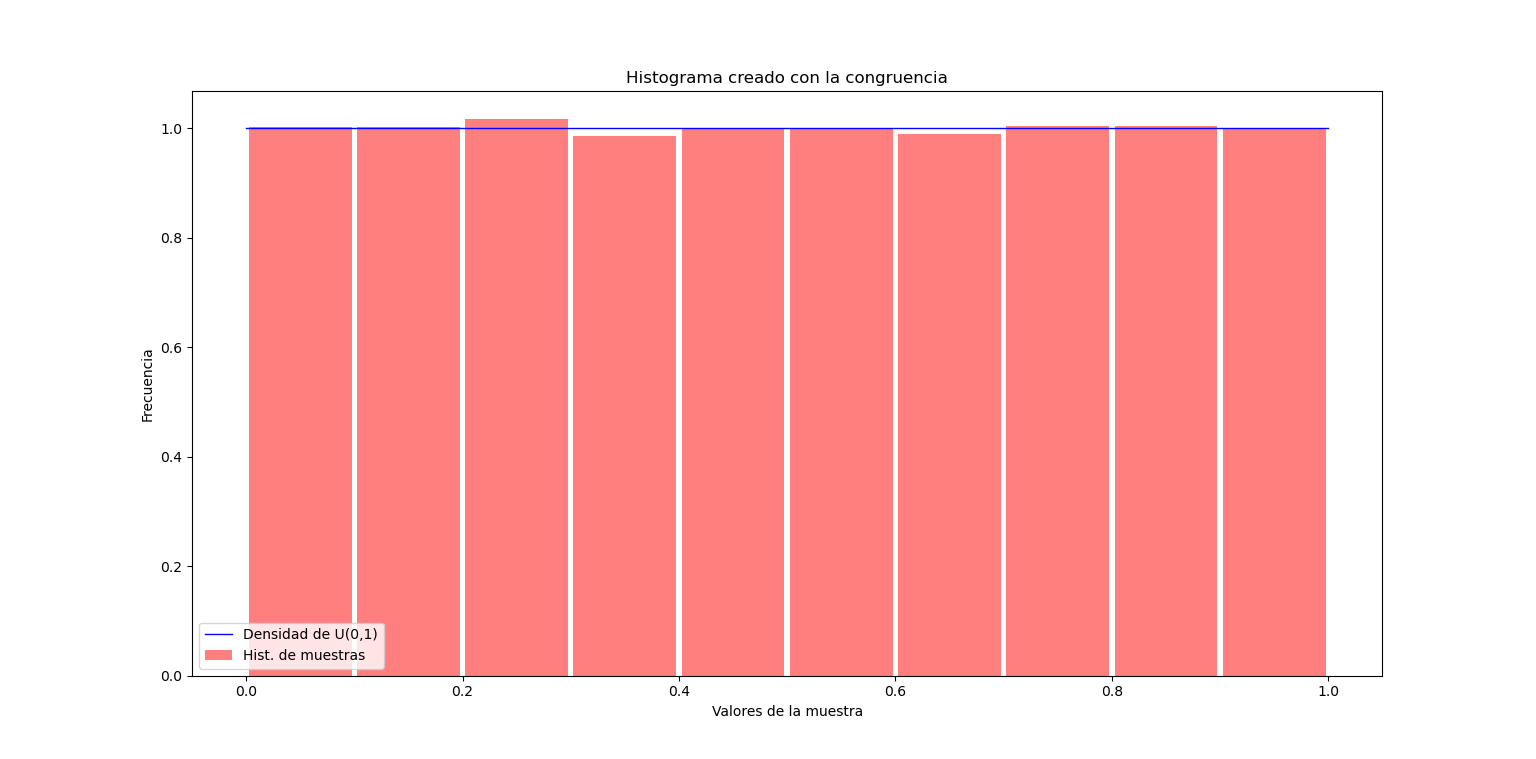
\includegraphics[width=0.9\linewidth]{3.png}
  \caption{Histograma de 100,000 muestras del algoritmo y su contraste con una densidad uniforme en (0,1). Vector inicial aleatorio}
\end{figure} 
\begin{figure}[h!]
\centering
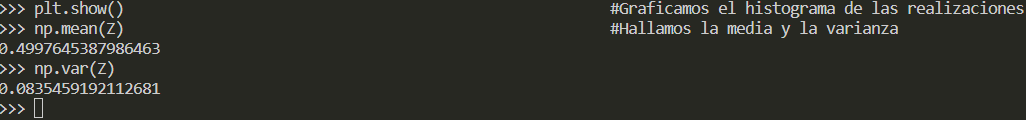
\includegraphics[width=0.9\linewidth]{4.png}
\caption{Media y varianza del muestreo anterior.}
\end{figure} 

Observamos nuevamente un buen comportamiento del histograma con respecto
a la densidad de una uniforme en (0,1). También observamos que el valor 
de la media muestral es de $\widehat{\mu}\approx0.49976$, bastante cercano al 
0.5 teórico, mientras que el valor de la varianza muestral es de 
$\widehat{\sigma}^2\approx0.083545$, que también aproxima bastante 
bien al valor $0.083333...$ teórico.

    \item[\textbf{3.}] ¿Cuál es el algoritmo que usa $scipy.stats.uniform$ para generar números aleatorios?
    ¿Cómo se pone la semilla? ¿Y en R?\\

    \textbf{Solución:} Esencialmente utiliza el generador de números pseudoaleatorios \textit{Mersenne Twister}. Este es un generador de números aleatorios 
    que utiliza el número primo de Mersenne $2^{19937}-1$, y que genera números enteros con base en una recurrencia lineal de matrices en el campo binario $F_2$,
    desarrollado por Makoto Matsumoto y Takuji Nishimura en 1997. Lo anterior ocurre por default a menos que se le indique lo contrario.\\

    Al abrir la documentación de $scipy.stats.uniform$, y dirigiéndonos al código fuente, entramos en la sección de la clase \textit{$uniform\_gen(rv\_continuous)$}, la cual 
    genera precisamente la variable aleatoria uniforme (ver \url{https://github.com/scipy/scipy/blob/v1.11.3/scipy/stats/_continuous_distns.py#L9766-L9946}). 
    Analizando el código, encontramos que el sufijo $\_rvs$ para la generación de la muestra aleatoria utiliza la función \textit{$random\_$state.uniform}.

    Nuevamente analizando la documentación de \textit{rando$m\_s$tate.uniform} (ver \url{https://numpy.org/devdocs/reference/random/legacy.html#numpy.random.RandomState}),
    notamos que esta viene de la función \textit{numpy.random.RandomState(arg)}, la cual es una
    función que tiene dentro de sí al generador de números pseudoaleatorios Mersenne Twister. Luego, lo que utiliza $scipy$ en última instancia para generar 
    números pseudoaleatorios es el generador anterior. No obstante, en el código fuente se nos indica que, si bien el generador por default es el anterior, 
    la nueva clase $numpy.random.Generator$ está recomendado como una alternativa que se ha de comenzar a utilizar en la medida de lo posible, y este
    generador de números aleatorios utiliza por defecto el algoritmo $PCG64$.
    \newline

    La semilla se puede colocar directamente en la parte $arg$ del código \textit{$random\_state.uniform(arg)$}, donde si no se coloca algo en el argumento (cualquier entero entre 0 y $2^{32}-1$),
    la semilla por defecto se coloca utilizando el tiempo interno de máquina. O bien, lo que se puede hacer es utilizar la función 
    \begin{verbatim}
      numpy.random.seed(arg),
    \end{verbatim}
    la cual directamente colocará la semilla que se le otorgue en el apartado $arg$ como la semilla que utilizará $scipy.stats.uniform$ a través
    de $numpy.random.RandomState(arg)$ como se vio antes.
    \newline

    En $R$, encontramos que hay 7 generadores de números pseudo-aleatorios, aunque el 
    que se usa por defecto nuevamente es Mersenne-Twister (ver \url{https://stat.ethz.ch/R-manual/R-devel/library/base/html/Random.html}),
    aunque su método de inicialización es propio de $R$.
    La semilla se coloca preferentemente (de acuerdo a la referencia inmediatamente anterior) utilizando
    \begin{verbatim}
      set.seed(arg),
    \end{verbatim}
    donde si $arg$ no es especificado, se utiliza también el tiempo interno de máquina.

    \item[\textbf{4.}] ¿En $scipy$ qué funciones hay para simular una variable aleatoria
    genérica discreta? ¿tienen preproceso? [1 punto]\\

    \textbf{Solución:} de la documentación de $scipy.stats$ (ver \url{https://docs.scipy.org/doc/scipy/reference/stats.html#discrete-distributions}),
    notamos que hay 19 funciones que generan 19 variables aleatorias, a saber, 
    
\begin{multicols*}{2}
      \begin{enumerate}
        \item Bernoulli (scipy.stats.bernoulli)
        \item Beta-bionomial (scipy.stats.betabinom)
        \item Binomial (scipy.stats.binom)
        \item Boltzmann (distribución exponencial truncada) (scipy.stats.boltzmann)
        \item Laplaciana (scipy.stats.dlaplace)
        \item Geométrica (scipy.stats.geom)
        \item Hipergeométrica (scipy.stats.hyoergeom)
        \item Logarítmica (scipy.stats.logser)
        \item Binomial Negativa (scipy.stats.nbinom)
        \columnbreak
        \item Hipergeométrica Fisher no centrada (scipy.stats.nchypergeom$\_$fisher)
        \item Hipergeométrica Wallenius no centrada (scipy.stats.nchypergeom$\_$wallenius)
        \item Hipergeométrica Negativa (scipy.stats.nchypergeom)
        \item Planck exponencial discreta (scipy.stats.planck)
        \item Poisson (scipy.stats.poisson)
        \item Uniforme (scipy.stats.randint)
        \item Skellam (scipy.stats.skellam)
        \item Yule-Simon (scipy.stats.yulesimon)
        \item Zipf (Zeta) (scipy.stats.zipf )
        \item Zipfian (scipy.stats.zipfian)f
      \end{enumerate}
\end{multicols*}
Como podemos ver, hay soporte para 19 variables aleatorias discretas.

\item[\textbf{5.}] Implementar el algoritmo Adaptive Rejection Sampling y simular una $Gamma(2,1)$, 10,000 muestras. ¿Cuando
    es conveniente dejar de adaptar la envolvente? (ver alg. A.7, p. 54 Robert y Casella, 2da ed.) [6 puntos]
    \newline

    \textbf{Solución: } este ejercicio se encuentra también en el script \textit{Ejercicios 2-5}, en la parte final del mismo. La idea es primero construir
    una función que calcule la envolvente, después pasarla a la forma exponencial, integrarla para obtener una función de densidad, y posteriormente 
    utilizar mezclas para muestrear de dicha función utilizando inversa generalizada. Finalmente, se utiliza el algoritmo de aceptación y rechazo para obtener 
    una muestra de la distribución g. Ya con dicha muestra, se añade el punto muestreado al algoritmo y se actualiza la envolvente.
\end{enumerate}
\end{document}